
\documentclass{article}
\usepackage{amsmath}
\usepackage{hyperref}
\usepackage{enumerate}
\usepackage{listings}
\usepackage{graphicx}
\usepackage{rotating}
\usepackage[flushleft]{threeparttable}
\graphicspath{ {../../plots/} }
\begin{document}
\newcommand{\ihs}{\mathrm{arcsinh}}
\title{Homework 2 \\ HW1, Econ 293}
\author{Luis Armona\footnote{Coding done in colloboration with Jack Blundell} \\ \href{mailto:larmona@stanford.edu}{larmona@stanford.edu} }
\maketitle
\section{Observational Study}
We return to the observational study we created in homework 1 of this class. Specifically, we take the randomized trial of promising various types of matching donations done in Karlan \& List's 2007 AER paper : ``Does Price Matter in Charitable Giving? Evidence from a Large-Scale Natural Field Experiment'', and add a selection component by dropping observations depending on their treatment status. Our selection rule, which keeps people (represented by an indicator $K_i$) in the sample with probability $\psi(X_i)$, takes a fairly complicated functional form:
\[
  \psi(X_i)= \begin{cases}
  	  (.01 + -0.01*\ihs(X_{3,i})^5 + \ihs(X_{3,i})^3)/300 & \text{if $W_i=1$} \\
	  (X_{2,s}+1)*(\arccos(X_{1,s})*\arctan(X_{1,s}) )/3 & \text{if $W_i=0$} \\ 
     0.5 & \text{if missing one of $X_{1,s},X_{2,s},X_{3,i}$}
      \end{cases} 
\]
Where $W_i$ is a treatment indicator, $X_{3,i}$ is the highest previous donation by the donor (\texttt{hpa}), $X_{2,s}$ is the number of cases the charity undertook in the state $s$ from 2004-05 (\texttt{cases}) , and $X_{2,s}$ is the state's voting share for George Bush in the 2004 presidential election (\texttt{perbush}), and $\ihs$ is the inverse hyperbolic sine function (e.g. $\ihs(X) = \log(X_{3,i} + \sqrt{X_{3,i} ^ 2 + 1}$).


From this Dropout rule we can recover the true propensity score as well for the selected sample:
\[
\rho(X_i) = P(W_i=1|K_i=1) = \frac{P(K_i=1|W_i=1)P(W_i=1) }{P(K_i=1|W_i=1)P(W_i=1) + P(K_i=1|W_i=0)P(W_i=0) }
\]
Before the analysis, I also split up our new quasi-experimental sample into test and training data sets (90\% train, 10\% test), as well as standardize all of the observable covariates/controls $\mathbf{X}$ to have mean 0 and standard deviation 1.
After installing the various packages required for this homework, I begin by running a propensity forest, which creates a forest trees that partition observations based on their observables and the probability of treatment (i.e. A regular random forest aiming to predict $W_i$). For our propensity forest estimation, for each tree build we sample the training data with replacement for a total of 1/2 the size of the training data, and randomly bag 1/3 of the covariates to avoid the individual trees looking to similar to each other / avoid overfitting. The risk criterion for each tree building is that of the regular partitioning tree, to  select each cut in order to minimize the misclassification rate of the treatment group within the resulting leaf nodes. After estimating a propensity tree, we can estimate an individual $i$'s conditional average treatment effect (CATE) within the tree $t$ by estimating the treatment effect within each node $l$ as a form of propensity matching:
\[\tau_{t,i} = \sum_{l} 1\{i\in l\} (\frac{1}{N_{t,l}}\sum_{i:W_i=1 \& i \in l} Y_i 
									- \frac{1}{N_{c,l}}\sum_{i:W_i=0 \& i \in l} Y_i) \]
and then averaging these node-specific CATEs across all trees to get an individual's overall propensity forest estimated CATE. I can also try to recover the original overall average treatment by taking the average of the propensity forest CATEs across indvididuals, similar to using matching methods to recover the ATE in an observational study. My estimate applying the forest onto the left-out test data is an ATE of $0.233$, which is decently close to the true ATE of $0.1536$, but still was outperformed by other methods from the previous problem set, such as double-robust methods. In Figure \ref{pfcate}, I plot the true propensity score against the propensity forest CATE's to detect heterogeneity by propensity of treatment in the response to treatment. The smoother fit here across the CATEs is a LOESS smoother. we see a large spread for high propensity individuals in their response to the treatment, and a relatively homogeneous response for low-propensity individuals.


I now estimate the CATEs in the observational study using the gradient forest package. using this package, one can estimate a causal forest by aggregating results from causal trees that individually at each partition decision maximize the heterogeneity in average treatment effects, by splitting on psuedo outcomes:
\[\rho_i =(W_i - \bar W_{\text{parent node}})( (Y_i - \bar Y_{\text{parent node}}) - (W_i - \bar W_{\text{parent node}})\tau_{\text{parent  node}}  ) \]

I do 2 versions of this gradient forest estimation, first by estimating on the raw data $Y_i$ and $W_i$, then by first residualizing both via a traditional CART regression forest both $Y_i$ and $W_i$ on observables $X_i$. I separately verify that computing residuals outside of the function (i.e. feeding it residuals) and using the built-in option \texttt{precompute.nuisance} yield extremely similar outcomes. The mean estimate of the ATE from the non-residualized gradient forest causal forest estimation is $0.236$, similar to our estimate ffrom the propensity forest. When I first residualize the gradient forest, I get an estimate ATE from the test data of $0.16$, which is actually the best performance we had across all of the attempted ATE recovery techniques. Figure \ref{gfcomp} shows the scatterplot of the residualized versus non-residualized estimate on the test data, as well as the 45 degree line. We see that the residualized versions estimate an average effect lower than the residualized version, and a slope relationship between the two estimates greater than 1. However, the residualized estimates also have a much larger variance (average of 0.47 in the residualized version, 0.22 on raw $Y_i$ and $W_i$).

\begin{figure}[!ht]
\center
\caption{CATEs by Propensity Score}
\label{pfcate}
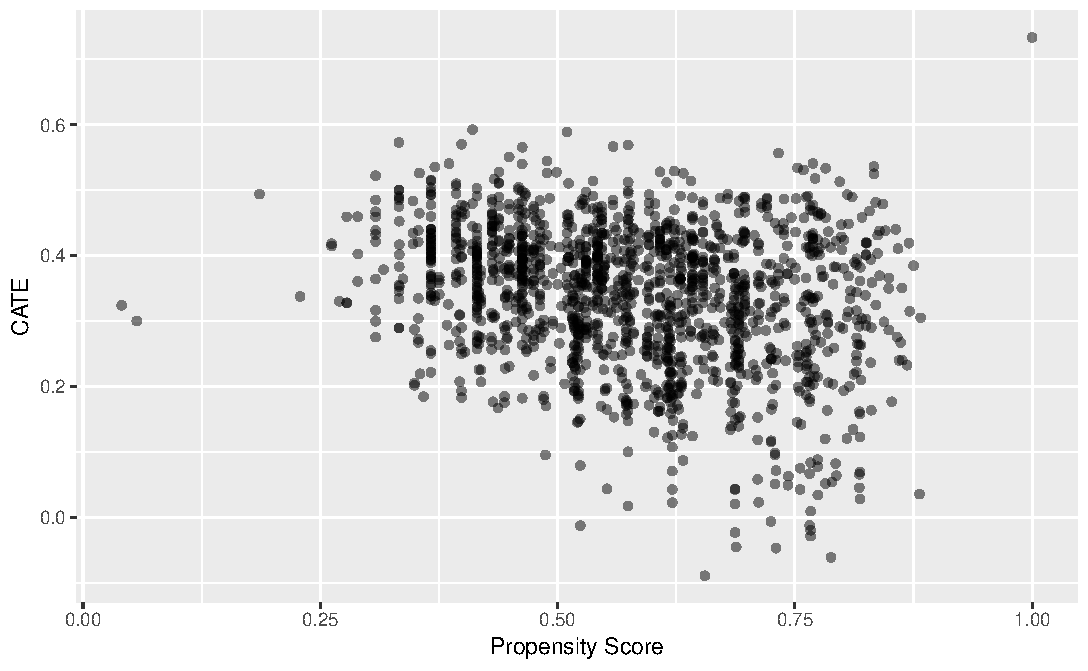
\includegraphics[scale=.7]{PFCATEvPS.pdf}
\end{figure}

\begin{figure}[!ht]
\center
\caption{Gradient Forest CATEs (Residualized vs Raw)}
\label{gfcomp}
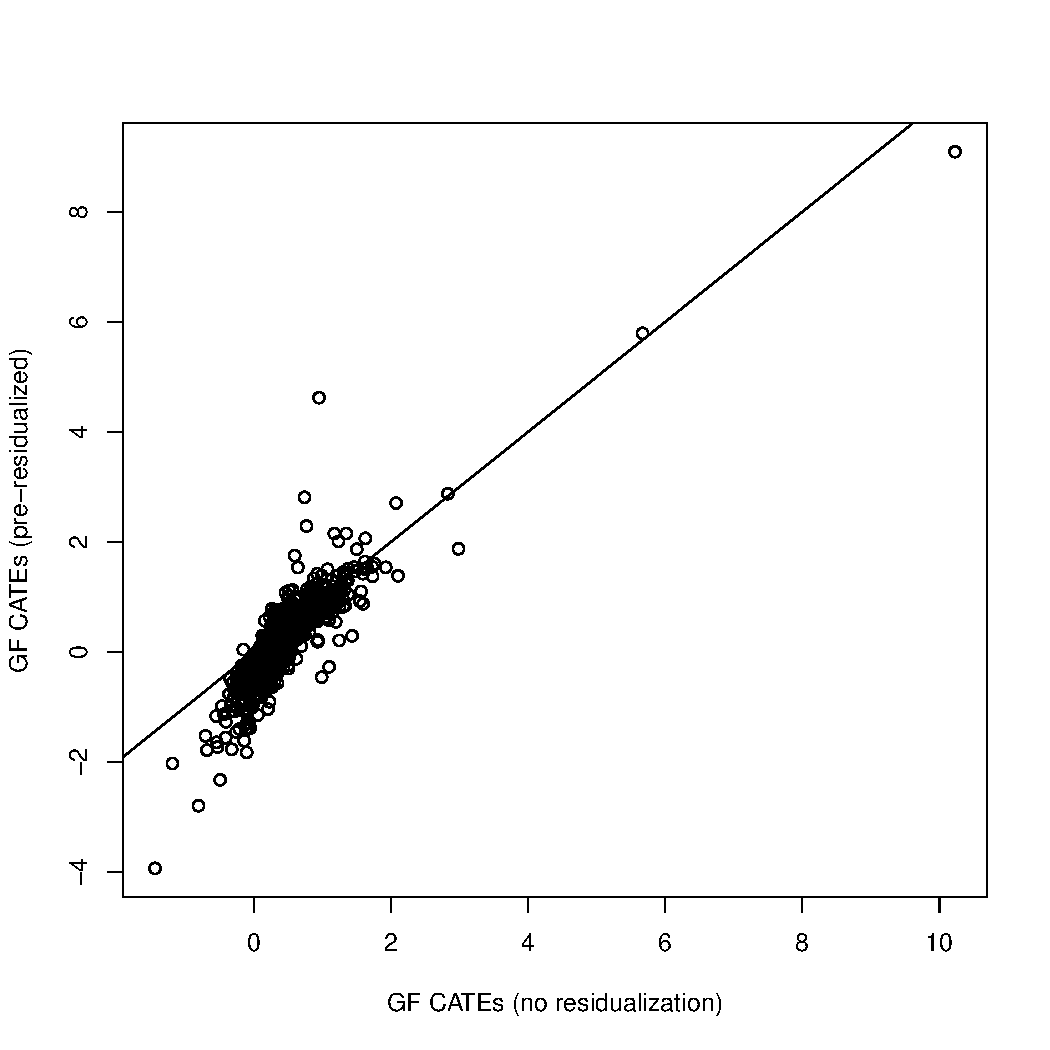
\includegraphics[scale=.7]{residGFcomp.pdf}
\end{figure}
\pagebreak
\clearpage
\section{Heterogeneity in Randomized Setting}
We now return to the randomized setting where treatment assignment $W_i$ is randomly allocated across the entire donor sample. As recommended, we split the sample evenly into 3 random samples, named A, B, and C. C is used as a left-out test dataset, A is the primary training set, and B is used for validation on the model trained by A. I begin by interacting treatment $W_i$ with all observables $X_i$ and estimate the lasso, while setting the penalty factor to zero on the uninteracted $W_i$, so it is never excluded. and estimate the best predictor of the outcome based on observables and their (linear) interaction with the treatment indicator. I then take these nonzero coefficients and perform post-OLS on all 3 samples and the union of the left out samples (B+C). I show below results for A and B+C. In both samples, we actually find some results consistent with the original paper: those in ``red'' (Republican-Leaning) counties were more effected by treatment (induced to pay more), while those in safer (recall the NGO doing the experiment is left-learning) blue counties paid less in response to treatment. While these are both directionally consistent findings, both interactions are insignificant in both the A and B+C samples.Outside of this, the regression output concerning treatment heterogeneity is largely inconsistent: many coefficients are different signs in each of the training and test sample, and hardly any are significant in either (with none being significant in both). Confidence intervals in both sets are not dramatically different. The MSE of the estimated treatment effects per individual from lasso (evaluated against $Y^* = -1^{W_i} Y_i / (W_i(p) + (1-W_i)(1-p))$, whose expectation is the individuals CATE, where $p$ is the overall propensity of treatment) is 317.29.

\input{lassopost_A.tex}
\input{lassopost_BC.tex}
\begin{figure}[!ht]
\center
\caption{Lasso Treatment Heterogeneity CV plot}
\label{lassocv}
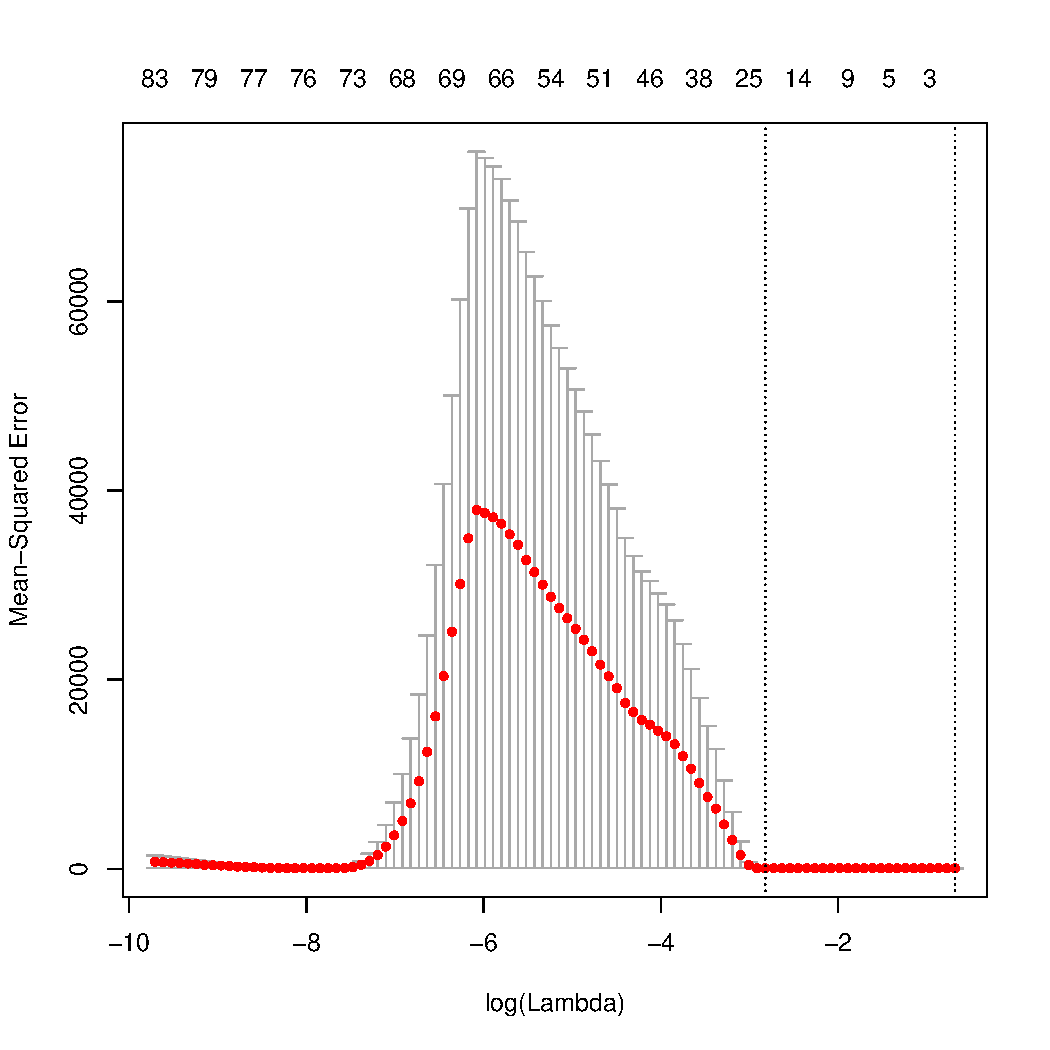
\includegraphics[scale=.7]{lasso_CV.pdf}
\end{figure}


I now move onto examining treatment heterogeneity via causal trees/ forests. First I estimate heterogeneity with a single causal tree, using sample A to choose the split,while estimating within leaf effects in sample B, using honest splitting/cross validation (i.e. using a left-out validation set for estimation of the heterogeneity within each split). For this and all following usages of forests, we use the traditional ``CT'' risk criterion with equal weighting $\alpha=.5$ of the greedy risk function and the honesty alteration. I also do the recommended splitting by bucket quantiles. The honest causal tree routine finds an optimal complexity penalty corresponding to 68 splits. The estimated decision tree is shown in Figure 4 \ref{honesttree}. I supplement this with a simple linear regression on the dummies for each of the 68 nodes estimated in the tree. See the R markup file for the full regression output for all samples. For the test leftout dataset (Sample B+C), only a few of the leaf nodes interacted with treatment (8 exactly) are found to be statistically significantly different from ATE (coefficient on uninteracted W), and if we account for multiple hypothesis testing, these are also unlikely to be significant post-correction. The MSE against $Y^*$ using the honest causal tree is 356.65, so it performs slightly worse than the lasso regression.
%\input{leafols_test.tex}

\begin{figure}[!ht]
\center
\caption{Estimated Treatment Heterogeneity Honest Causal Tree }
\label{honesttree}
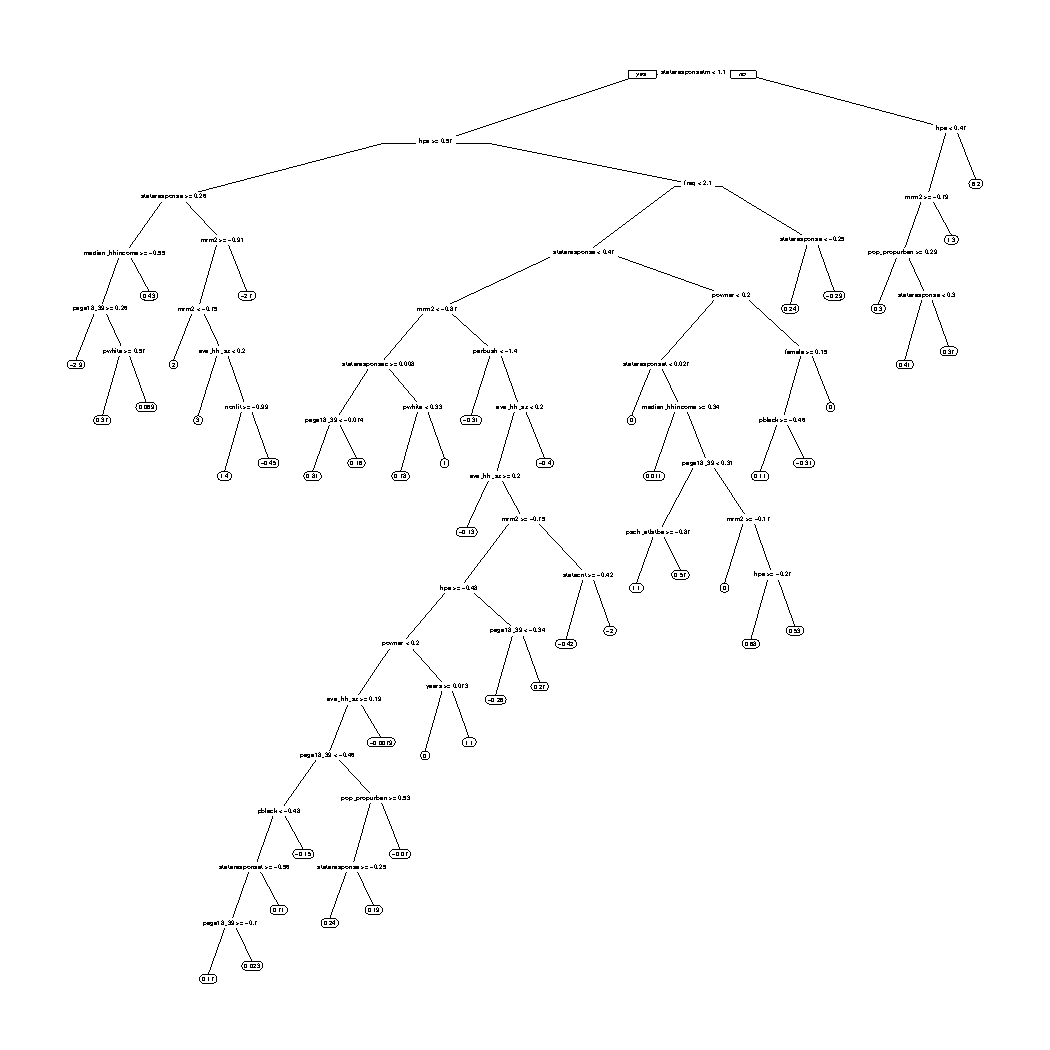
\includegraphics[scale=1]{honestCT.pdf}
\end{figure}
 

 I now turn to estimating a causal forest ( an ensemble of honest causal trees). using the \texttt{causalForest} function from Athey's \texttt{causalTree} package. For reasons I am unable to diagnose, the \texttt{causalForest} function does not appear to function properly: the forest mostly estimates degenerate trees (one node, mean treatment). resulting in a de-facto CATE of $0$ for all individuals. What is particularly strange is I run into no issues estimating the CATE of individuals using the \texttt{causal.forest} function from Stefan Wager's \texttt{gradient.forst} package , passing the identical corresponding arguments (honest splitting, min size of nodes, etc.). After experimenting with the options, I find that lowering the sample size bagged for each tree increasing the number of splits, but these are still very close to zero within leaves. The MSE of this virtually zero ATE for all individuals on $Y^*$ is 356.3425.


  Thus, I now turn to the gradient forest package for estimating the causal forest / visualizing the heterogeneity with a heatmap. First, as a baseline I do gradient forest without residualizing the outcome (note we do not need to residualize $W$ since it is now randomly allocated). I recieve an MSE against $Y^*$ of 356.07, which is not much better than predicting zero everywhere for a CATE. For the residualized version, I pre-residualzie the outcome $Y$ in the A+B sample using a regression forest, then estimate the causal forest on this orthogonalized outcome. The gradient forest  uncovers a rich amount of heterogeneity, with CATEs as extreme as +/- 20, but most of the CATE density mass is much closer to zero (See Figure \ref{gfdens}). I supplement this with a direct look at two covariates of interest and how treatment heterogeneity occurs on this dimension: the donor's previous contribution and \% in the donor's state that voted for President George W. Bush in the 2004 Election. Intuitively, we might expect that those who donated larger amounts in the past would react more strongly in magnitude to treatment since they were already more likely to donate a larger amount, assuming there is positive correlation between past and future donation amounts. In a different vein, the paper originally using the data uncovered notable heterogeneity by right-leaning nature of the donor's state. Figure \ref{heatmap} plots the CATE along both of these dimensions. note the axes are not linear but instead spaced along the unique values of each found in the data. We find that the most affected donors by treatment are exactly those who contributed large amounts in the past (around $\$225$ and simultaneously live in a heavily Republican state where Bush gathered 60\% of the presidential vote). on the other hand, the most unaffected are those who are large donors and live in highly Democratic-leaning states, as demonstrated by the southeast corner of the heatmap. Finally, we find an MSE against $Y^*$ of 356.67. which is basically comparable to the zero ATE prediction.

At the end of the exercise, gradient forest and causal trees are fairly successful at uncovering heterogeneity. The lasso also accomplishes this but the results are inconsistent and more difficult to understand in the causal sense. As I discussed, there appears to be a bug in the \texttt{causalForest} function. The heterogeneity from the residualized gradient causal forest appears is on average larger in magnitude, as is evident in Figure \ref{gfres_random}. The lasso by far performs the best in minimizing MSE of $Y^*$, where the other heterogeneity effect estimators do not do noticeably better than the prediction of zero ATE (i.e. $\hat Y_i^* = Y)i$.

\begin{figure}[!ht]
\center
\caption{Density of CATEs from Residualized Gradient Forest}
\label{gfdens}
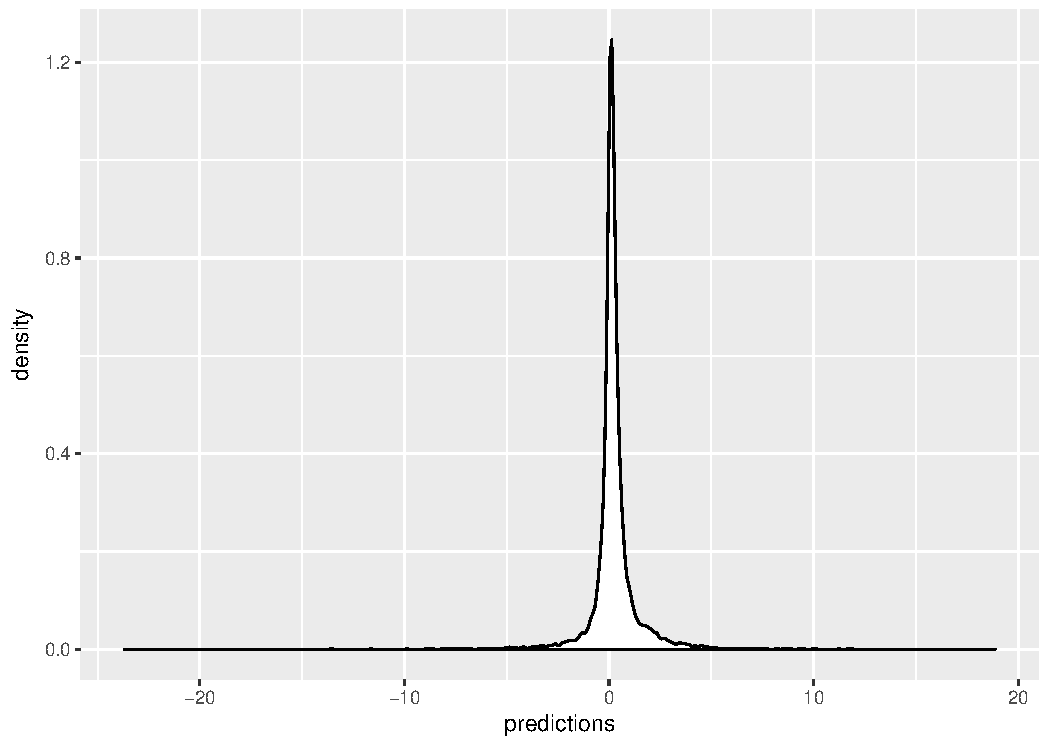
\includegraphics[scale=.8]{cate_gf.pdf}
\end{figure}
 
 \begin{figure}[!ht]
\center
\caption{Heatmap of CATEs by Previous Contribution and \% votes for Republicans}
\label{heatmap}
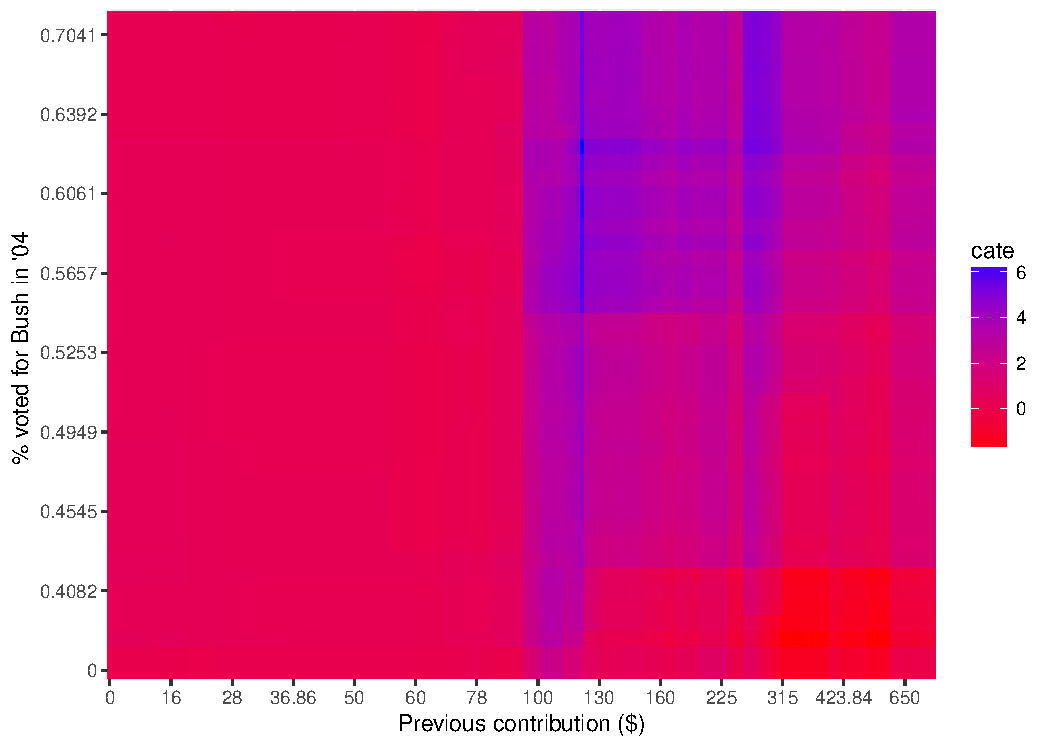
\includegraphics[scale=.8]{heatmap.pdf}
\end{figure}
 
  \begin{figure}[!ht]
\center
\caption{Gradient Forest CATEs (Residualized vs Raw) in the Randomized Experiment}
\label{gfres_random}
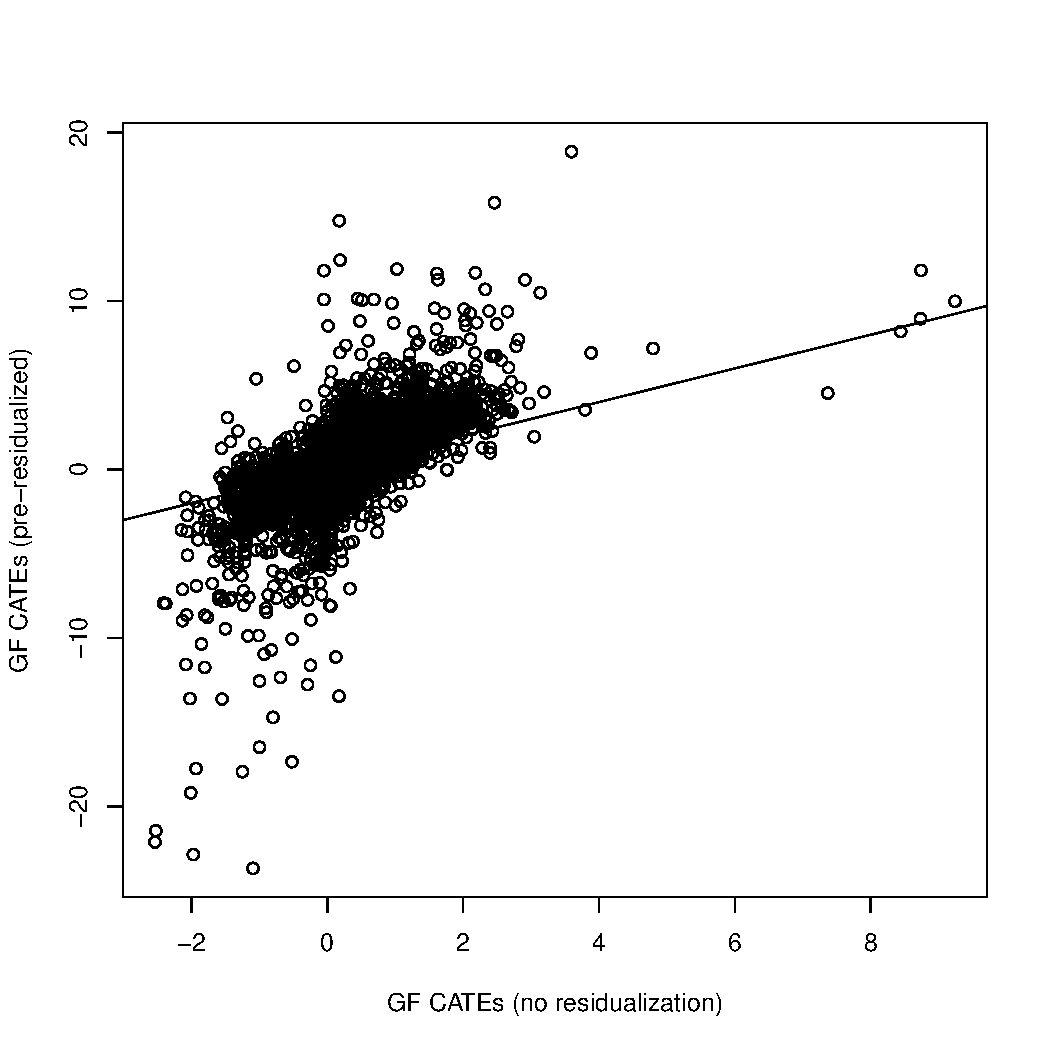
\includegraphics[scale=.8]{residGFcomp_random.pdf}
\end{figure}
 

\end{document}